\documentclass[11pt]{article}

\usepackage[a4paper,margin=0.85in]{geometry}
\usepackage{amsmath,amssymb,mathtools}
\usepackage{enumitem}
\usepackage{tikz}
\usepackage{pgfplots}
\pgfplotsset{compat=1.18}
\usetikzlibrary{arrows.meta,calc,positioning,patterns,decorations.pathreplacing,shapes.geometric}
\usepackage[most]{tcolorbox}
\usepackage{xcolor}
\usepackage{hyperref}
\usepackage{microtype}
\usepackage{booktabs}

\definecolor{navy}{HTML}{102A43}
\definecolor{ashblue}{HTML}{1D4E89}
\definecolor{softblue}{HTML}{EAF4FF}
\definecolor{softgreen}{HTML}{EAF7ED}
\definecolor{softred}{HTML}{FFF0F0}
\definecolor{softgray}{HTML}{F7F9FB}
\definecolor{lineorange}{HTML}{D97706}
\definecolor{linegreen}{HTML}{2F855A}
\definecolor{linered}{HTML}{C53030}

\hypersetup{colorlinks=true, linkcolor=ashblue, urlcolor=ashblue}
\setlength{\parindent}{0pt}
\setlength{\parskip}{6pt}
\setlist[enumerate]{itemsep=4pt, topsep=4pt}

\newcommand{\R}{\mathbb{R}}
\newcommand{\norm}[1]{\left\lVert #1 \right\rVert}
\newcommand{\abs}[1]{\left\lvert #1 \right\rvert}
\newcommand{\ip}[2]{#1\cdot #2}
\newcommand{\dd}{\,d}
\newcommand{\e}{\mathrm e}

\newtcolorbox{strategybox}[1][]{
  enhanced,
  colback=softblue,
  colframe=ashblue!70!black,
  boxrule=0.7pt,
  arc=2mm,
  left=2mm,right=2mm,top=1mm,bottom=1mm,
  title=Strategy,#1
}
\newtcolorbox{answerbox}[1][]{
  enhanced,
  colback=softgreen,
  colframe=linegreen!70!black,
  boxrule=0.7pt,
  arc=2mm,
  left=2mm,right=2mm,top=1mm,bottom=1mm,
  title=Final answer,#1
}
\newtcolorbox{warningbox}[1][]{
  enhanced,
  colback=softred,
  colframe=linered!70!black,
  boxrule=0.7pt,
  arc=2mm,
  left=2mm,right=2mm,top=1mm,bottom=1mm,
  title=Important check,#1
}

\title{\textbf{Multivariable Calculus: Problem Set 4}\\Detailed Assignment-Style Solutions}
\author{Prepared solution set}
\date{}

\begin{document}
\maketitle

\begin{center}
\begin{tcolorbox}[enhanced,width=0.92\textwidth,colback=softgray,colframe=navy!60!black,arc=2mm,boxrule=0.7pt]
This solution set gives explicit computations, path choices, continuity arguments, and derivative definitions.  The word ``limit exists along a path'' always means the one-variable limit obtained after restricting the function to that path.  The full multivariable limit is stronger: it must give the same value along every path approaching the point.
\end{tcolorbox}
\end{center}

\tableofcontents
\newpage

\section{Problem 1: Unit tangent, unit normal, and binormal}

\begin{strategybox}
For a regular curve \(\mathbf r(t)\), the Frenet vectors are computed by
\[
\mathbf T(t)=\frac{\mathbf r'(t)}{\norm{\mathbf r'(t)}},\qquad
\mathbf N(t)=\frac{\mathbf T'(t)}{\norm{\mathbf T'(t)}}\quad(\mathbf T'(t)\neq 0),\qquad
\mathbf B(t)=\mathbf T(t)\times \mathbf N(t).
\]
So the method is: differentiate \(\mathbf r\), normalize to get \(\mathbf T\), differentiate \(\mathbf T\), normalize to get \(\mathbf N\), and finally take the cross product.
\end{strategybox}

\begin{center}
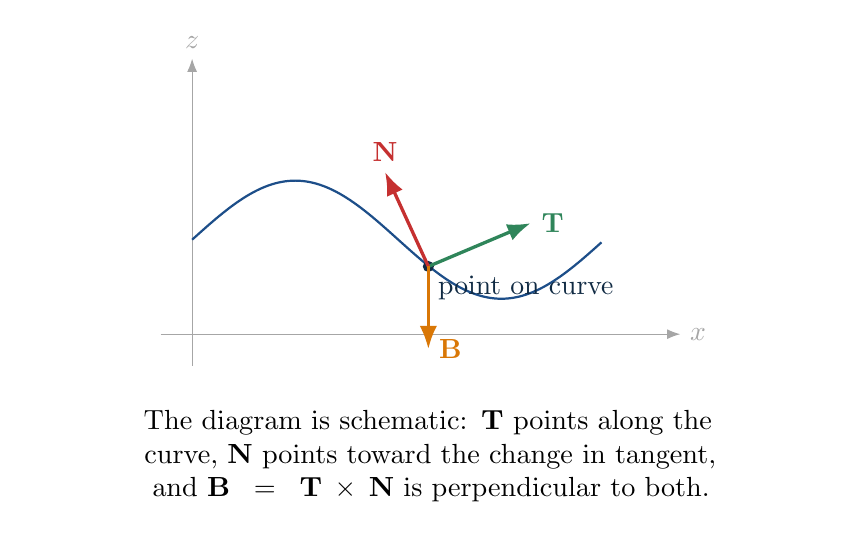
\begin{tikzpicture}[scale=1.0,>=Latex]
  \draw[->,gray!70] (-0.4,0) -- (6.2,0) node[right] {$x$};
  \draw[->,gray!70] (0,-0.4) -- (0,3.5) node[above] {$z$};
  \draw[thick,ashblue,domain=0:5.2,samples=120,smooth] plot ({\x},{1.2+0.75*sin(1.2*\x r)});
  \coordinate (P) at (3,0.86);
  \fill[navy] (P) circle (2pt) node[below right] {point on curve};
  \draw[->,very thick,linegreen] (P) -- ++(1.3,0.55) node[right] {$\mathbf T$};
  \draw[->,very thick,linered] (P) -- ++(-0.55,1.2) node[above] {$\mathbf N$};
  \draw[->,very thick,lineorange] (P) -- ++(0.0,-1.05) node[right] {$\mathbf B$};
  \node[align=center,text width=0.82\textwidth] at (3,-1.55) {The diagram is schematic: \(\mathbf T\) points along the curve, \(\mathbf N\) points toward the change in tangent, and \(\mathbf B=\mathbf T\times\mathbf N\) is perpendicular to both.};
\end{tikzpicture}
\end{center}

\subsection{1(i) \(\mathbf r(t)=(\cos t,t,\sin t)\), at \(t=0\)}

First compute the velocity:
\[
\mathbf r'(t)=(-\sin t,1,\cos t).
\]
Its speed is
\[
\norm{\mathbf r'(t)}=\sqrt{\sin^2t+1+\cos^2t}=\sqrt{2}.
\]
Therefore
\[
\mathbf T(t)=\frac{1}{\sqrt2}(-\sin t,1,\cos t).
\]
At \(t=0\),
\[
\mathbf T(0)=\left(0,\frac{1}{\sqrt2},\frac{1}{\sqrt2}\right).
\]
Now differentiate \(\mathbf T\):
\[
\mathbf T'(t)=\frac{1}{\sqrt2}(-\cos t,0,-\sin t).
\]
Thus
\[
\norm{\mathbf T'(t)}=\frac{1}{\sqrt2}\sqrt{\cos^2t+\sin^2t}=\frac{1}{\sqrt2}.
\]
So
\[
\mathbf N(t)=(-\cos t,0,-\sin t),
\]
and hence
\[
\mathbf N(0)=(-1,0,0).
\]
Finally,
\[
\mathbf B(0)=\mathbf T(0)\times \mathbf N(0)
=\left(0,\frac{1}{\sqrt2},\frac{1}{\sqrt2}\right)\times(-1,0,0)
=\left(0,-\frac{1}{\sqrt2},\frac{1}{\sqrt2}\right).
\]

\begin{answerbox}
\[
\boxed{\mathbf T(0)=\left(0,\frac1{\sqrt2},\frac1{\sqrt2}\right),\quad
\mathbf N(0)=(-1,0,0),\quad
\mathbf B(0)=\left(0,-\frac1{\sqrt2},\frac1{\sqrt2}\right).}
\]
\end{answerbox}

\subsection{1(ii) \(\mathbf r(t)=(\cos t,\sin t,\ln(\cos t))\), at \(t=0\)}

The curve is defined near \(t=0\) because \(\cos t>0\) near \(0\). We compute
\[
\mathbf r'(t)=(-\sin t,\cos t,-\tan t).
\]
Near \(0\), \(\sec t>0\), and
\[
\norm{\mathbf r'(t)}
=\sqrt{\sin^2t+\cos^2t+\tan^2t}
=\sqrt{1+\tan^2t}
=\sec t.
\]
Therefore
\[
\mathbf T(t)=\frac{(-\sin t,\cos t,-\tan t)}{\sec t}
=(-\sin t\cos t,\cos^2t,-\sin t).
\]
At \(t=0\),
\[
\mathbf T(0)=(0,1,0).
\]
Now differentiate:
\[
\mathbf T'(t)=(-\cos^2t+\sin^2t,-2\sin t\cos t,-\cos t).
\]
At \(t=0\),
\[
\mathbf T'(0)=(-1,0,-1),
\qquad
\norm{\mathbf T'(0)}=\sqrt2.
\]
Thus
\[
\mathbf N(0)=\frac{1}{\sqrt2}(-1,0,-1)
=\left(-\frac1{\sqrt2},0,-\frac1{\sqrt2}\right).
\]
Finally,
\[
\mathbf B(0)=\mathbf T(0)\times\mathbf N(0)
=(0,1,0)\times\left(-\frac1{\sqrt2},0,-\frac1{\sqrt2}\right)
=\left(-\frac1{\sqrt2},0,\frac1{\sqrt2}\right).
\]

\begin{answerbox}
\[
\boxed{\mathbf T(0)=(0,1,0),\quad
\mathbf N(0)=\left(-\frac1{\sqrt2},0,-\frac1{\sqrt2}\right),\quad
\mathbf B(0)=\left(-\frac1{\sqrt2},0,\frac1{\sqrt2}\right).}
\]
\end{answerbox}

\subsection{1(iii) \(\mathbf r(t)=\left(t,\frac12t^2,t^2\right)\), at \(t=0\)}

We compute
\[
\mathbf r'(t)=(1,t,2t),
\qquad
\norm{\mathbf r'(t)}=\sqrt{1+t^2+4t^2}=\sqrt{1+5t^2}.
\]
Thus
\[
\mathbf T(t)=\frac{(1,t,2t)}{\sqrt{1+5t^2}}.
\]
At \(t=0\),
\[
\mathbf T(0)=(1,0,0).
\]
To find \(\mathbf N(0)\), we need \(\mathbf T'(0)\). Since the derivative of the denominator factor contributes zero at \(t=0\),
\[
\mathbf T'(0)=(0,1,2).
\]
Therefore
\[
\norm{\mathbf T'(0)}=\sqrt{0^2+1^2+2^2}=\sqrt5,
\]
and
\[
\mathbf N(0)=\left(0,\frac1{\sqrt5},\frac2{\sqrt5}\right).
\]
Finally,
\[
\mathbf B(0)=\mathbf T(0)\times \mathbf N(0)
=(1,0,0)\times\left(0,\frac1{\sqrt5},\frac2{\sqrt5}\right)
=\left(0,-\frac2{\sqrt5},\frac1{\sqrt5}\right).
\]

\begin{answerbox}
\[
\boxed{\mathbf T(0)=(1,0,0),\quad
\mathbf N(0)=\left(0,\frac1{\sqrt5},\frac2{\sqrt5}\right),\quad
\mathbf B(0)=\left(0,-\frac2{\sqrt5},\frac1{\sqrt5}\right).}
\]
\end{answerbox}

\newpage
\section{Problem 2: Limits}

\subsection{2(i) Indicator function of the line \(y=2x\)}

The function is
\[
f(x,y)=
\begin{cases}
2,& y=2x,\\
0,& \text{otherwise.}
\end{cases}
\]
The support of the function is exactly the line \(y=2x\). Therefore, if a path approaches a point while avoiding this line except possibly at the endpoint, the path-limit is \(0\). If the path lies on the line \(y=2x\), the path-limit is \(2\).

\begin{center}
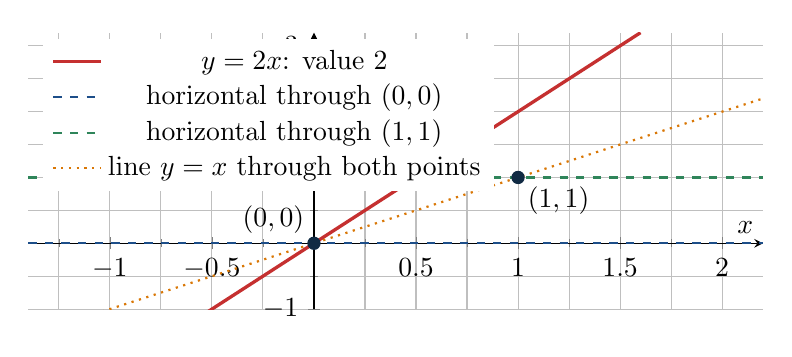
\begin{tikzpicture}[scale=1.0,>=Latex]
  \begin{axis}[
    width=0.9\textwidth,height=0.42\textwidth,
    axis lines=middle,
    xmin=-1.4,xmax=2.2,ymin=-1.0,ymax=3.2,
    xlabel={$x$},ylabel={$y$},
    grid=both, minor tick num=1,
    legend style={at={(0.02,0.98)},anchor=north west,draw=none,fill=white},
  ]
    \addplot[domain=-1.4:1.6,samples=2,very thick,linered] {2*x};
    \addlegendentry{$y=2x$: value $2$}
    \addplot[domain=-1.4:2.2,samples=2,thick,ashblue,dashed] {0};
    \addlegendentry{horizontal through $(0,0)$}
    \addplot[domain=-1.4:2.2,samples=2,thick,linegreen,dashed] {1};
    \addlegendentry{horizontal through $(1,1)$}
    \addplot[domain=-1.4:2.2,samples=2,thick,lineorange,dotted] {x};
    \addlegendentry{line $y=x$ through both points}
    \addplot[only marks,mark=*,mark size=2.2pt,navy] coordinates {(0,0) (1,1)};
    \node[anchor=south east] at (axis cs:0,0) {$(0,0)$};
    \node[anchor=north west] at (axis cs:1,1) {$(1,1)$};
  \end{axis}
\end{tikzpicture}
\end{center}

\subsubsection*{At \((0,0)\)}

\textbf{(a) Line parallel to the \(x\)-axis.} The horizontal line through \((0,0)\) is \(y=0\). Along this line,
\[
f(x,0)=2 \quad\text{only if}\quad 0=2x,
\]
which happens only at \(x=0\). For every punctured point near \((0,0)\) on this path, \(x\neq0\), so \(f(x,0)=0\). Hence
\[
\lim_{x\to0} f(x,0)=0.
\]

\textbf{(b) Line parallel to the \(y\)-axis.} The vertical line through \((0,0)\) is \(x=0\). Along this line,
\[
f(0,y)=2 \quad\text{only if}\quad y=2(0)=0.
\]
For every punctured point near \((0,0)\), \(y\neq0\), so \(f(0,y)=0\). Therefore
\[
\lim_{y\to0} f(0,y)=0.
\]

\textbf{(c) Lines parallel to \(y=mx\).} Through \((0,0)\), this line is \(y=mx\). Then
\[
f(x,mx)=
\begin{cases}
2,& mx=2x,\\
0,& mx\neq2x.
\end{cases}
\]
For \(x\neq0\), the condition \(mx=2x\) is equivalent to \(m=2\). Hence
\[
\lim_{x\to0}f(x,mx)=
\begin{cases}
2,&m=2,\\
0,&m\neq2.
\end{cases}
\]
Because different lines give different limits, the full limit at \((0,0)\) does not exist.

\begin{answerbox}
At \((0,0)\), the horizontal and vertical path-limits are both \(0\), but the line \(y=2x\) gives limit \(2\). Therefore
\[
\boxed{\lim_{(x,y)\to(0,0)} f(x,y)\text{ does not exist}.}
\]
\end{answerbox}

\subsubsection*{At \((1,1)\)}

The point \((1,1)\) is not on \(y=2x\), because \(1\neq2\). In fact, the distance from \((1,1)\) to the line \(y=2x\) is positive:
\[
\frac{|1-2|}{\sqrt{1+(-2)^2}}=\frac1{\sqrt5}.
\]
So there is a small ball around \((1,1)\) that does not meet the special line \(y=2x\). Inside that ball, \(f=0\) identically.

\textbf{(a) Horizontal line.} The horizontal line is \(y=1\). It meets \(y=2x\) only at \(x=1/2\), which is not near \(x=1\). Thus
\[
\lim_{x\to1} f(x,1)=0.
\]

\textbf{(b) Vertical line.} The vertical line is \(x=1\). It meets \(y=2x\) only at \(y=2\), which is not near \(y=1\). Thus
\[
\lim_{y\to1} f(1,y)=0.
\]

\textbf{(c) Line with slope \(m\) through \((1,1)\).} Such a line is
\[
y-1=m(x-1),\qquad\text{or}\qquad y=mx-m+1.
\]
No such line can equal \(y=2x\), because \((1,1)\notin y=2x\). It may intersect \(y=2x\) at at most one point away from \((1,1)\), but a sufficiently small neighborhood around \((1,1)\) avoids that point. Hence every such line-limit is \(0\).

\begin{answerbox}
At \((1,1)\), the function is identically \(0\) in a small enough neighborhood of the point. Therefore
\[
\boxed{\lim_{(x,y)\to(1,1)} f(x,y)=0.}
\]
\end{answerbox}

\subsection{2(ii) Constructing examples in \(\R^3\)}

\subsubsection*{2(ii)(a): Limit exists along one coordinate axis but not the other}

For an example where the limit exists along the \(x\)-axis but does not exist along the \(y\)-axis, define
\[
f(x,y,z)=
\begin{cases}
\sin(1/y),& y\neq0,\\
0,&y=0.
\end{cases}
\]
Along the \(x\)-axis, points have the form \((t,0,0)\), so
\[
f(t,0,0)=0\quad\Rightarrow\quad \lim_{t\to0}f(t,0,0)=0.
\]
Along the \(y\)-axis, points have the form \((0,t,0)\), so
\[
f(0,t,0)=\sin(1/t),
\]
which has no limit as \(t\to0\). Thus the required behavior occurs.

For the reverse behavior, define
\[
g(x,y,z)=
\begin{cases}
\sin(1/x),&x\neq0,\\
0,&x=0.
\end{cases}
\]
Then the limit along the \(y\)-axis exists and equals \(0\), while the limit along the \(x\)-axis does not exist.

\begin{answerbox}
One example is \(f(x,y,z)=\sin(1/y)\) for \(y\neq0\), and \(f=0\) for \(y=0\).  The reverse example is obtained by replacing \(y\) with \(x\).
\end{answerbox}

\subsubsection*{2(ii)(b): Coordinate-axis limits exist, but a line limit fails}

Define
\[
f(x,y,z)=
\begin{cases}
\sin(1/x),& y=x,\ x\neq0,\\
0,&\text{otherwise.}
\end{cases}
\]
Along the \(x\)-axis, points are \((t,0,0)\). For \(t\neq0\), \(0\neq t\), so the point is not on \(y=x\), hence
\[
f(t,0,0)=0.
\]
Thus the \(x\)-axis limit is \(0\). Along the \(y\)-axis, points are \((0,t,0)\). For \(t\neq0\), \(t\neq0=x\), so again
\[
f(0,t,0)=0.
\]
Thus the \(y\)-axis limit is \(0\). But along the line \(y=x\), using points \((t,t,0)\),
\[
f(t,t,0)=\sin(1/t),
\]
which has no limit as \(t\to0\).

\begin{answerbox}
\[
\boxed{
 f(x,y,z)=
\begin{cases}
\sin(1/x),&y=x,\ x\neq0,\\
0,&\text{otherwise}
\end{cases}}
\]
has coordinate-axis limits, but no limit along the line \(y=x\).
\end{answerbox}

\subsubsection*{2(ii)(c): All straight-line limits exist, but a curved path gives a different value}

Define
\[
f(x,y,z)=
\begin{cases}
\dfrac{x^2y}{x^4+y^2},&(x,y)\neq(0,0),\\[6pt]
0,&(x,y)=(0,0).
\end{cases}
\]
The variable \(z\) is irrelevant here. Along a line \(y=mx\),
\[
f(x,mx,z)=\frac{x^2(mx)}{x^4+m^2x^2}
=\frac{mx}{x^2+m^2}\quad(m\neq0),
\]
and this tends to \(0\) as \(x\to0\). For \(m=0\), the function is also \(0\). Therefore every line \(y=mx\) gives limit \(0\).

However, along the curve \(y=x^2\),
\[
f(x,x^2,0)=\frac{x^2x^2}{x^4+x^4}=\frac12.
\]
Thus the curved path gives limit \(1/2\), while all the straight lines considered above give limit \(0\).

\begin{center}
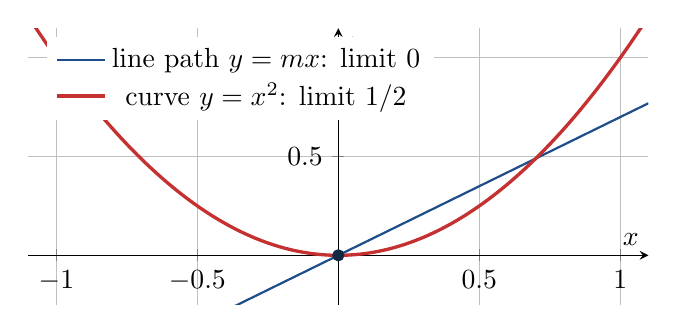
\begin{tikzpicture}[>=Latex,scale=1]
\begin{axis}[
  width=0.78\textwidth,height=0.42\textwidth,
  axis lines=middle,xmin=-1.1,xmax=1.1,ymin=-0.25,ymax=1.15,
  xlabel={$x$},ylabel={$y$},grid=both,
  legend style={draw=none,fill=white,at={(0.03,0.97)},anchor=north west}
]
\addplot[domain=-1.1:1.1,samples=2,ashblue,thick] {0.7*x};
\addlegendentry{line path $y=mx$: limit $0$}
\addplot[domain=-1.1:1.1,samples=160,linered,very thick] {x^2};
\addlegendentry{curve $y=x^2$: limit $1/2$}
\addplot[only marks,mark=*,mark size=2pt,navy] coordinates {(0,0)};
\end{axis}
\end{tikzpicture}
\end{center}

\begin{answerbox}
This example proves that checking all straight lines is not enough to prove a multivariable limit exists.
\end{answerbox}

\subsection{2(iii) Indicator function of the parabola \(y=x^2\)}

The function is
\[
f(x,y)=
\begin{cases}
2,&y=x^2,\\
0,&\text{otherwise.}
\end{cases}
\]
The support is exactly the parabola \(y=x^2\).

\begin{center}
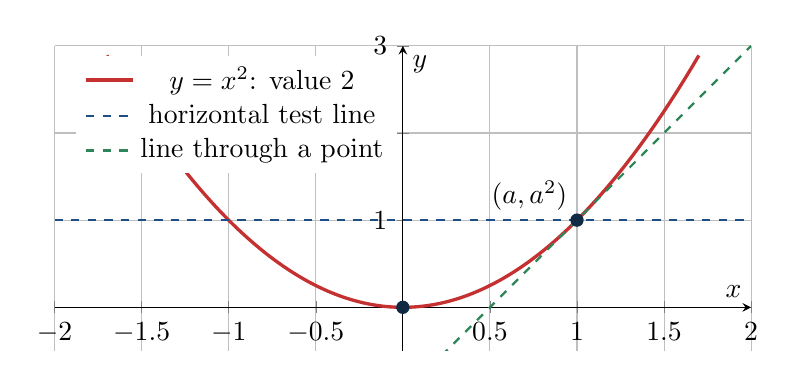
\begin{tikzpicture}[scale=1,>=Latex]
\begin{axis}[
  width=0.86\textwidth,height=0.45\textwidth,
  axis lines=middle,xmin=-2,xmax=2,ymin=-0.5,ymax=3.0,
  xlabel={$x$},ylabel={$y$},grid=both,
  legend style={draw=none,fill=white,at={(0.03,0.97)},anchor=north west}
]
\addplot[domain=-1.7:1.7,samples=160,linered,very thick] {x^2};
\addlegendentry{$y=x^2$: value $2$}
\addplot[domain=-2:2,samples=2,ashblue,dashed,thick] {1};
\addlegendentry{horizontal test line}
\addplot[domain=-2:2,samples=2,linegreen,dashed,thick] {2*x-1};
\addlegendentry{line through a point}
\addplot[only marks,mark=*,mark size=2.2pt,navy] coordinates {(1,1) (0,0)};
\node[anchor=south east] at (axis cs:1,1) {$(a,a^2)$};
\end{axis}
\end{tikzpicture}
\end{center}

Let \(P=(a,b)\).

\textbf{Case 1: \(P\notin\{(x,y):y=x^2\}\).} Then \(b\neq a^2\). Since the parabola is a closed curve and \(P\) is not on it, there is a small ball around \(P\) that does not meet the parabola. In that ball, \(f=0\). Therefore all path-limits, and in fact the full limit, equal \(0\).

\textbf{Case 2: \(P=(a,a^2)\) lies on the parabola.} Along the parabola itself, approaching \(P\), the value is always \(2\). Hence the curved-path limit along \(y=x^2\) is \(2\). Now check the requested straight paths.

\textbf{(a) Horizontal line.} The horizontal line through \(P\) is \(y=a^2\). It meets the parabola where
\[
x^2=a^2,
\]
so \(x=a\) or \(x=-a\). Near the point \((a,a^2)\), the only possible intersection is the point itself. Therefore, on the punctured horizontal path sufficiently near \(P\), the function equals \(0\), and the horizontal line-limit is \(0\).

\textbf{(b) Vertical line.} The vertical line through \(P\) is \(x=a\). It meets the parabola only at \(y=a^2\). Thus, on the punctured vertical path near \(P\), \(f=0\). The vertical line-limit is \(0\).

\textbf{(c) Lines parallel to \(y=mx\).} A line with slope \(m\) through \((a,a^2)\) is
\[
y-a^2=m(x-a).
\]
Intersect it with the parabola:
\[
x^2-a^2=m(x-a).
\]
Factor:
\[
(x-a)(x+a)=m(x-a),
\]
so
\[
(x-a)(x+a-m)=0.
\]
Thus one intersection is \(x=a\), namely the point \(P\). The other possible intersection is \(x=m-a\), which is a fixed point. Unless it is the same as \(a\), it is away from \(P\); if it is the same as \(a\), then the line is tangent and still meets the parabola only at \(P\) locally. Therefore, every straight-line path through \(P\) has punctured values \(0\) near \(P\), and every such line-limit is \(0\).

\begin{answerbox}
For points not on the parabola, the full limit is \(0\). For points on the parabola, every requested straight-line limit is \(0\), but the path along the parabola gives \(2\). Therefore the full limit does not exist at any point of the parabola.
\end{answerbox}

\subsection{2(iv) Direct limit computations}

\subsubsection*{2(iv)(a) \(\displaystyle \lim_{(x,y)\to(0,0)}\frac{xy}{\sqrt{x^2+y^2}}\)}

Use the inequality
\[
2\abs{xy}\leq x^2+y^2.
\]
Then
\[
\left|\frac{xy}{\sqrt{x^2+y^2}}\right|
\leq \frac{x^2+y^2}{2\sqrt{x^2+y^2}}
=\frac12\sqrt{x^2+y^2}.
\]
As \((x,y)\to(0,0)\), the right side tends to \(0\). Therefore, by the squeeze theorem,
\[
\boxed{\lim_{(x,y)\to(0,0)}\frac{xy}{\sqrt{x^2+y^2}}=0.}
\]

\subsubsection*{2(iv)(b) \(\displaystyle \lim_{(x,y)\to(0,0)}\frac{x^4+y^4}{x^2+y^2}\)}

Since
\[
x^4+y^4\leq (x^2+y^2)^2,
\]
we get
\[
0\leq \frac{x^4+y^4}{x^2+y^2}\leq x^2+y^2.
\]
As \((x,y)\to(0,0)\), the right side tends to \(0\). Hence
\[
\boxed{\lim_{(x,y)\to(0,0)}\frac{x^4+y^4}{x^2+y^2}=0.}
\]

\subsubsection*{2(iv)(c) \(\displaystyle \lim_{(x,y)\to(0,0)}\frac{x^2y\e^y}{x^4+4y^2}\)}

Here the denominator contains \(x^4\) and \(y^2\), so the suspicious path is \(y=kx^2\). Try two choices.

Along \(y=x^2\),
\[
\frac{x^2(x^2)\e^{x^2}}{x^4+4x^4}
=\frac{x^4\e^{x^2}}{5x^4}
=\frac{\e^{x^2}}{5}\to\frac15.
\]
Along \(y=-x^2\),
\[
\frac{x^2(-x^2)\e^{-x^2}}{x^4+4x^4}
=-\frac{\e^{-x^2}}{5}\to -\frac15.
\]
The two path-limits are different. Therefore the full limit does not exist.

\begin{answerbox}
\[
\boxed{\lim_{(x,y)\to(0,0)}\frac{x^2y\e^y}{x^4+4y^2}\text{ does not exist}.}
\]
\end{answerbox}

\subsection{2(v) The function \(\displaystyle f(x,y)=\frac{x^2-y^2}{x^2+y^2}\)}

Along the line \(y=mx\), put \((x,y)=(h,mh)\). Then
\[
f(h,mh)=\frac{h^2-m^2h^2}{h^2+m^2h^2}
=\frac{1-m^2}{1+m^2}.
\]
Therefore
\[
\lim_{h\to0}f(h,mh)=\frac{1-m^2}{1+m^2}.
\]
This limit exists for each fixed \(m\), but it depends on \(m\). For example,
\[
m=0\Rightarrow \lim=1,
\qquad
m=1\Rightarrow \lim=0.
\]
Because different paths give different limiting values, the full limit at the origin does not exist.

\begin{answerbox}
The origin cannot be assigned any value that makes \(f\) continuous, because continuity would require the full limit at the origin to exist. It does not.
\end{answerbox}

\subsection{2(vi) Unequal iterated limits}

Take
\[
f(x,y)=
\begin{cases}
\dfrac{x^2-y^2}{x^2+y^2},&(x,y)\neq(0,0),\\[6pt]
0,&(x,y)=(0,0).
\end{cases}
\]
First compute the inner limit with respect to \(y\). For fixed \(x\neq0\),
\[
\lim_{y\to0}f(x,y)=\frac{x^2}{x^2}=1.
\]
Therefore
\[
\lim_{x\to0}\lim_{y\to0}f(x,y)=\lim_{x\to0}1=1.
\]
Now reverse the order. For fixed \(y\neq0\),
\[
\lim_{x\to0}f(x,y)=\frac{-y^2}{y^2}=-1.
\]
Therefore
\[
\lim_{y\to0}\lim_{x\to0}f(x,y)=\lim_{y\to0}(-1)=-1.
\]
So the two iterated limits exist but are unequal.

\begin{answerbox}
\[
\boxed{\lim_{x\to0}\lim_{y\to0}f(x,y)=1\neq -1=\lim_{y\to0}\lim_{x\to0}f(x,y).}
\]
\end{answerbox}

If the full two-variable limit \(\lim_{(x,y)\to(0,0)}f(x,y)=L\) exists, and the two iterated limits are defined, then both iterated limits must equal \(L\). The reason is that for all points sufficiently close to \((0,0)\), the values of \(f(x,y)\) must be close to \(L\), no matter how the point approaches \((0,0)\). Hence the iterated limits cannot produce two different values.

\newpage
\section{Problem 3: Continuity}

\subsection{3(i) Continuity of \(f(x)=\norm{x}\)}

Let \(a\in\R^m\). We need to show
\[
\norm{x}\to\norm{a}\quad\text{as}\quad x\to a.
\]
The reverse triangle inequality gives
\[
\abs{\norm{x}-\norm{a}}\leq\norm{x-a}.
\]
Therefore, if \(\norm{x-a}<\delta\), then
\[
\abs{f(x)-f(a)}<\delta.
\]
Given \(\varepsilon>0\), choose \(\delta=\varepsilon\). This proves continuity at \(a\). Since \(a\) was arbitrary, \(f\) is continuous on \(\R^m\).

\begin{answerbox}
\[
\boxed{x\mapsto\norm{x}\text{ is continuous on }\R^m.}
\]
\end{answerbox}

\subsection{3(ii) Continuity of coordinate projection \(f_i(x)=x^{(i)}\)}

Let \(a=(a^{(1)},\dots,a^{(m)})\). Then
\[
\abs{f_i(x)-f_i(a)}=\abs{x^{(i)}-a^{(i)}}\leq\norm{x-a}.
\]
Given \(\varepsilon>0\), choose \(\delta=\varepsilon\). If \(\norm{x-a}<\delta\), then
\[
\abs{f_i(x)-f_i(a)}<\varepsilon.
\]
Thus every coordinate projection is continuous.

\begin{answerbox}
\[
\boxed{f_i(x)=x^{(i)}\text{ is continuous for every }1\leq i\leq m.}
\]
\end{answerbox}

\subsection{3(iii) Continuity of \(f(x)=c\cdot x\)}

Let \(a\in\R^m\). Then
\[
f(x)-f(a)=c\cdot x-c\cdot a=c\cdot(x-a).
\]
By the Cauchy-Schwarz inequality,
\[
\abs{f(x)-f(a)}=\abs{c\cdot(x-a)}\leq \norm{c}\norm{x-a}.
\]
If \(c=0\), then \(f\) is constant and continuous. If \(c\neq0\), choose
\[
\delta=\frac{\varepsilon}{\norm{c}}.
\]
Then \(\norm{x-a}<\delta\) implies \(\abs{f(x)-f(a)}<\varepsilon\). Hence \(f\) is continuous.

\begin{answerbox}
\[
\boxed{x\mapsto c\cdot x\text{ is continuous on }\R^m.}
\]
\end{answerbox}

\subsection{3(iv) Continuity of a vector-valued function from continuous components}

Let
\[
f(x)=(f_1(x),f_2(x)),
\]
where \(f_1,f_2:\R\to\R\) are continuous. Fix \(a\in\R\). Since \(f_1\) and \(f_2\) are continuous at \(a\), for a given \(\varepsilon>0\), choose \(\delta_1>0\) such that
\[
|x-a|<\delta_1\Rightarrow |f_1(x)-f_1(a)|<\frac{\varepsilon}{\sqrt2},
\]
and choose \(\delta_2>0\) such that
\[
|x-a|<\delta_2\Rightarrow |f_2(x)-f_2(a)|<\frac{\varepsilon}{\sqrt2}.
\]
Let \(\delta=\min\{\delta_1,\delta_2\}\). Then
\[
\norm{f(x)-f(a)}
=\sqrt{(f_1(x)-f_1(a))^2+(f_2(x)-f_2(a))^2}
<\sqrt{\frac{\varepsilon^2}{2}+\frac{\varepsilon^2}{2}}
=\varepsilon.
\]
So \(f\) is continuous.

\begin{answerbox}
\[
\boxed{(f_1,f_2)\text{ is continuous whenever }f_1\text{ and }f_2\text{ are continuous.}}
\]
\end{answerbox}

\subsection{3(v) Continuity of \(f(x,y,z)=(f_1(z),f_2(x))\)}

Let \((a,b,c)\in\R^3\). We need to show
\[
(f_1(z),f_2(x))\to (f_1(c),f_2(a))
\]
as \((x,y,z)\to(a,b,c)\). Since \(f_1\) is continuous at \(c\), \(z\to c\) implies \(f_1(z)\to f_1(c)\). Since \(f_2\) is continuous at \(a\), \(x\to a\) implies \(f_2(x)\to f_2(a)\). The variable \(y\) does not affect the output. Therefore both components are continuous, so the vector-valued map is continuous.

\begin{answerbox}
\[
\boxed{f(x,y,z)=(f_1(z),f_2(x))\text{ is continuous on }\R^3.}
\]
\end{answerbox}

\subsection{3(vi) Quotient of continuous functions}

Let \(f,g:A\to\R\) be continuous and let \(x_0\in A\) satisfy \(g(x_0)\neq0\). We first prove that \(g\) stays nonzero near \(x_0\).

Since \(g\) is continuous at \(x_0\), choose \(\delta>0\) such that
\[
\norm{x-x_0}<\delta\quad\Rightarrow\quad |g(x)-g(x_0)|<\frac{|g(x_0)|}{2}.
\]
Then
\[
|g(x)|\geq |g(x_0)|-|g(x)-g(x_0)|>
|g(x_0)|-\frac{|g(x_0)|}{2}
=\frac{|g(x_0)|}{2}>0.
\]
Thus \(g(x)\neq0\) for all \(x\in A\cap B_\delta(x_0)\).

Now define \(q(x)=1/g(x)\) near \(x_0\). Then
\[
\left|q(x)-q(x_0)\right|
=\left|\frac{1}{g(x)}-\frac{1}{g(x_0)}\right|
=\frac{|g(x)-g(x_0)|}{|g(x)||g(x_0)|}.
\]
Near \(x_0\), the denominator is bounded below by \(|g(x_0)|^2/2\), and the numerator tends to \(0\). Hence \(q\) is continuous at \(x_0\). Since \(f\) is continuous and products of continuous functions are continuous,
\[
\frac{f}{g}=f\cdot\frac1g
\]
is continuous at \(x_0\).

\begin{answerbox}
\[
\boxed{\frac{f}{g}\text{ is continuous at }x_0\text{ whenever }g(x_0)\neq0.}
\]
\end{answerbox}

\subsection{3(vii) Sets of continuity}

\subsubsection*{3(vii)(a)}
\[
f(x,y,z)=\left(\sin(x^2+5yz),\sqrt{1-\cos^2x},\e^{yz}\right).
\]
The first component is a composition of polynomials and sine, hence continuous. The third component is a composition of multiplication and exponential, hence continuous. For the second component,
\[
\sqrt{1-\cos^2x}=\sqrt{\sin^2x}=|\sin x|,
\]
which is continuous on \(\R\). Therefore the whole vector-valued function is continuous everywhere.

\begin{answerbox}
\[
\boxed{\text{Continuity set} = \R^3.}
\]
\end{answerbox}

\subsubsection*{3(vii)(b)}
\[
f(x,y,z)=\frac{x^2+y^2+\log(x^2+y^2)}{x+y+z-1}.
\]
The logarithm requires
\[
x^2+y^2>0,
\]
so \((x,y)\neq(0,0)\). The denominator requires
\[
x+y+z-1\neq0.
\]
On the set where both conditions hold, the numerator and denominator are continuous and the denominator is nonzero. Hence the quotient is continuous exactly there.

\begin{answerbox}
\[
\boxed{\text{Continuity set}=\bigl\{(x,y,z)\in\R^3:(x,y)\neq(0,0),\ x+y+z\neq1\bigr\}.}
\]
\end{answerbox}

\subsubsection*{3(vii)(c)}
\[
f(x,y)=
\begin{cases}
\dfrac{xy}{x^2+xy+y^2},&(x,y)\neq(0,0),\\[6pt]
0,&(x,y)=(0,0).
\end{cases}
\]
First note that
\[
x^2+xy+y^2=\left(x+\frac y2\right)^2+\frac34y^2.
\]
This is strictly positive for every \((x,y)\neq(0,0)\). Therefore \(f\) is a quotient of continuous functions away from the origin, so it is continuous on \(\R^2\setminus\{(0,0)\}\).

At the origin, check two paths. Along \(y=0\),
\[
f(x,0)=0.
\]
Along \(y=x\),
\[
f(x,x)=\frac{x^2}{x^2+x^2+x^2}=\frac13.
\]
The two path-limits differ. Therefore the limit at the origin does not exist, so \(f\) is not continuous at the origin.

\begin{answerbox}
\[
\boxed{\text{Continuity set}=\R^2\setminus\{(0,0)\}.}
\]
\end{answerbox}

\newpage
\section{Problem 4: Partial derivatives}

\subsection{4(i) First-order partial derivatives}

\subsubsection*{4(i)(a) \(\displaystyle f(x,y)=\int_x^y\cos(\e^t)\dd t\)}

Use the fundamental theorem of calculus with variable limits. Differentiating with respect to the lower limit gives a negative sign; differentiating with respect to the upper limit gives a positive sign:
\[
f_x(x,y)=-\cos(\e^x),
\qquad
f_y(x,y)=\cos(\e^y).
\]

\subsubsection*{4(i)(b) \(f(x,y)=\e^{xy}\sin y\)}

With respect to \(x\), \(\sin y\) is constant:
\[
f_x(x,y)=y\e^{xy}\sin y.
\]
With respect to \(y\), use the product rule:
\[
f_y(x,y)=x\e^{xy}\sin y+\e^{xy}\cos y
=\e^{xy}(x\sin y+
\cos y).
\]

\subsubsection*{4(i)(c) \(\displaystyle f(x,y,z)=\sqrt{\sin^2x+\sin^2y+\sin^2z}\)}

Let
\[
S(x,y,z)=\sin^2x+\sin^2y+\sin^2z.
\]
At points where \(S>0\), the chain rule gives
\[
f_x=\frac{\sin x\cos x}{\sqrt{S}},
\qquad
f_y=\frac{\sin y\cos y}{\sqrt{S}},
\qquad
f_z=\frac{\sin z\cos z}{\sqrt{S}}.
\]
At points where \(S=0\), all of \(x,y,z\) are integer multiples of \(\pi\). At such a point, for example in the \(x\)-direction,
\[
f(x_0+h,y_0,z_0)=|\sin(x_0+h)|=|\sin h|.
\]
Then
\[
\frac{f(x_0+h,y_0,z_0)-f(x_0,y_0,z_0)}{h}=\frac{|\sin h|}{h},
\]
which has different one-sided behavior. Hence the partial derivative does not exist there. The same reasoning applies to the other variables.

\begin{answerbox}
At points where \(S>0\),
\[
\boxed{f_x=\frac{\sin x\cos x}{\sqrt S},\quad
f_y=\frac{\sin y\cos y}{\sqrt S},\quad
f_z=\frac{\sin z\cos z}{\sqrt S}.}
\]
At points where \(S=0\), the first-order partial derivatives do not exist.
\end{answerbox}

\subsubsection*{4(i)(d) \(f(x,y,z)=x^ay^bz^c\)}

Assuming the variables lie in a domain where these powers are differentiable, the power rule gives
\[
f_x=a x^{a-1}y^bz^c,
\qquad
f_y=b x^ay^{b-1}z^c,
\qquad
f_z=c x^ay^bz^{c-1}.
\]

\subsection{4(ii) Mixed second-order partial derivatives}

\subsubsection*{4(ii)(a) \(f(x,y)=\e^{xy}\sin y\)}

From above,
\[
f_x=y\e^{xy}\sin y.
\]
Differentiate with respect to \(y\):
\[
f_{xy}
=\e^{xy}\sin y+y\left(x\e^{xy}\sin y+\e^{xy}\cos y\right)
=\e^{xy}\left(\sin y+xy\sin y+y\cos y\right).
\]
Also
\[
f_y=\e^{xy}(x\sin y+\cos y).
\]
Differentiate with respect to \(x\):
\[
f_{yx}=y\e^{xy}(x\sin y+\cos y)+\e^{xy}\sin y
=\e^{xy}\left(xy\sin y+y\cos y+\sin y\right).
\]
Therefore
\[
\boxed{f_{xy}=f_{yx}.}
\]

\subsubsection*{4(ii)(b) \(f(x,y)=x^2+y^2\sin(xy)\)}

First,
\[
f_x=2x+y^3\cos(xy).
\]
Then
\[
f_{xy}=3y^2\cos(xy)-xy^3\sin(xy).
\]
Next,
\[
f_y=2y\sin(xy)+xy^2\cos(xy).
\]
Differentiate with respect to \(x\):
\[
f_{yx}=2y^2\cos(xy)+y^2\cos(xy)-xy^3\sin(xy)
=3y^2\cos(xy)-xy^3\sin(xy).
\]
Thus
\[
\boxed{f_{xy}=f_{yx}=3y^2\cos(xy)-xy^3\sin(xy).}
\]

\subsubsection*{4(ii)(c) \(\displaystyle f(\mathbf x)=\sum_{i=1}^n\sum_{j=1}^n a_{ij}x_ix_j\), with \(a_{ij}=a_{ji}\)}

Let \(\mathbf x=(x_1,\dots,x_n)\). For a fixed index \(k\), the derivative with respect to \(x_k\) receives contributions from terms where \(i=k\) and from terms where \(j=k\):
\[
\frac{\partial f}{\partial x_k}
=\sum_{j=1}^n a_{kj}x_j+\sum_{i=1}^n a_{ik}x_i.
\]
Since \(a_{ik}=a_{ki}\), this becomes
\[
\frac{\partial f}{\partial x_k}=2\sum_{j=1}^n a_{kj}x_j.
\]
Now differentiate with respect to \(x_\ell\):
\[
\frac{\partial^2 f}{\partial x_\ell\partial x_k}=2a_{k\ell}.
\]
Similarly,
\[
\frac{\partial^2 f}{\partial x_k\partial x_\ell}=2a_{\ell k}=2a_{k\ell}.
\]
Therefore the mixed partial derivatives are equal.

\begin{answerbox}
\[
\boxed{\frac{\partial^2 f}{\partial x_\ell\partial x_k}
=\frac{\partial^2 f}{\partial x_k\partial x_\ell}=2a_{k\ell}.}
\]
\end{answerbox}

\subsection{4(iii) Examples involving mixed partial derivatives}

\subsubsection*{4(iii)(a) Mixed partials exist at the origin but are not equal}

Define
\[
f(x,y)=
\begin{cases}
\dfrac{xy(x^2-y^2)}{x^2+y^2},&(x,y)\neq(0,0),\\[6pt]
0,&(x,y)=(0,0).
\end{cases}
\]
Compute \(f_x(0,y)\). For \(y\neq0\),
\[
f_x(0,y)=\lim_{h\to0}\frac{f(h,y)-f(0,y)}{h}
=\lim_{h\to0}\frac{hy(h^2-y^2)}{(h^2+y^2)h}
=\lim_{h\to0} y\frac{h^2-y^2}{h^2+y^2}
=-y.
\]
Also \(f_x(0,0)=0\). Therefore
\[
f_{xy}(0,0)=\lim_{k\to0}\frac{f_x(0,k)-f_x(0,0)}{k}
=\lim_{k\to0}\frac{-k}{k}=-1.
\]
Now compute \(f_y(x,0)\). For \(x\neq0\),
\[
f_y(x,0)=\lim_{k\to0}\frac{f(x,k)-f(x,0)}{k}
=\lim_{k\to0}\frac{xk(x^2-k^2)}{(x^2+k^2)k}
=\lim_{k\to0}x\frac{x^2-k^2}{x^2+k^2}
=x.
\]
Also \(f_y(0,0)=0\). Therefore
\[
f_{yx}(0,0)=\lim_{h\to0}\frac{f_y(h,0)-f_y(0,0)}{h}
=\lim_{h\to0}\frac{h}{h}=1.
\]

\begin{answerbox}
\[
\boxed{f_{xy}(0,0)=-1\neq1=f_{yx}(0,0).}
\]
\end{answerbox}

\subsubsection*{4(iii)(b) Mixed partials exist, are equal, and are continuous}

Take the polynomial
\[
f(x,y)=x^2y^2.
\]
Then
\[
f_x=2xy^2,
\qquad
f_{xy}=4xy.
\]
Also
\[
f_y=2x^2y,
\qquad
f_{yx}=4xy.
\]
Both mixed partials are equal everywhere, and \(4xy\) is continuous everywhere.

\begin{answerbox}
\[
\boxed{f(x,y)=x^2y^2\text{ works, with }f_{xy}=f_{yx}=4xy.}
\]
\end{answerbox}

\subsubsection*{4(iii)(c) Mixed partials exist and are equal at the origin, but are not continuous}

Define
\[
f(x,y)=
\begin{cases}
\dfrac{x^2y^2}{x^2+y^2},&(x,y)\neq(0,0),\\[6pt]
0,&(x,y)=(0,0).
\end{cases}
\]
At the origin, first observe that
\[
f_x(0,y)=0,
\qquad
f_y(x,0)=0.
\]
Therefore
\[
f_{xy}(0,0)=0,
\qquad
f_{yx}(0,0)=0.
\]
So the mixed partials exist and are equal at the origin.

For \((x,y)\neq(0,0)\), direct differentiation gives
\[
f_{xy}(x,y)=\frac{8x^3y^3}{(x^2+y^2)^3}.
\]
Along the line \(y=x\),
\[
f_{xy}(x,x)=\frac{8x^6}{(2x^2)^3}=1.
\]
Along the line \(y=0\),
\[
f_{xy}(x,0)=0.
\]
Thus \(f_{xy}(x,y)\) does not tend to \(0=f_{xy}(0,0)\) as \((x,y)\to(0,0)\). Hence the mixed partial derivative is not continuous at the origin.

\begin{answerbox}
\[
\boxed{f(x,y)=\frac{x^2y^2}{x^2+y^2}\text{ for }(x,y)\neq0,\ f(0,0)=0\text{ works}.}
\]
\end{answerbox}

\newpage
\section{Problem 5: Directional derivatives}

\begin{strategybox}
For \(f:\R^n\to\R\), the partial derivative in the \(i\)-th coordinate direction at \(a\) is
\[
\frac{\partial f}{\partial x_i}(a)=\lim_{h\to0}\frac{f(a+h e_i)-f(a)}{h},
\]
when the limit exists. The directional derivative at \(a\) in the unit direction \(u\) is
\[
D_u f(a)=\lim_{h\to0}\frac{f(a+hu)-f(a)}{h},
\]
when the limit exists as a finite two-sided limit.
\end{strategybox}

\subsection{5(i) \(f(\mathbf x)=\norm{\mathbf x}^2\) on \(\R^3\)}

Write \(\mathbf x=(x_1,x_2,x_3)\). Then
\[
f(\mathbf x)=x_1^2+x_2^2+x_3^2.
\]

\textbf{(a) At the origin.} For the \(i\)-th partial derivative,
\[
\frac{\partial f}{\partial x_i}(0)
=\lim_{h\to0}\frac{f(he_i)-f(0)}{h}
=\lim_{h\to0}\frac{h^2}{h}
=\lim_{h\to0}h=0.
\]
So all partial derivatives exist at the origin and equal \(0\).

\textbf{(b) At any nonzero vector.} Since \(f\) is a polynomial,
\[
\frac{\partial f}{\partial x_i}(\mathbf x)=2x_i.
\]
This formula is valid at every point, including nonzero vectors.

\textbf{(c) Directional derivative at the origin.} Let \(u\) be a unit vector. Then
\[
D_u f(0)=\lim_{h\to0}\frac{f(hu)-f(0)}{h}
=\lim_{h\to0}\frac{\norm{hu}^2}{h}
=\lim_{h\to0}\frac{h^2\norm{u}^2}{h}
=\lim_{h\to0}h=0.
\]

\begin{answerbox}
\[
\boxed{\nabla f(\mathbf x)=2\mathbf x,
\qquad \nabla f(0)=0,
\qquad D_u f(0)=0.}
\]
\end{answerbox}

\subsection{5(ii) \(f(\mathbf x)=a\cdot\mathbf x\) on \(\R^3\)}

Let \(a=(a_1,a_2,a_3)\) and \(\mathbf x=(x_1,x_2,x_3)\). Then
\[
f(\mathbf x)=a_1x_1+a_2x_2+a_3x_3.
\]

\textbf{(a) At the origin.} For the \(i\)-th coordinate direction,
\[
\frac{\partial f}{\partial x_i}(0)
=\lim_{h\to0}\frac{f(he_i)-f(0)}{h}
=\lim_{h\to0}\frac{a_i h}{h}=a_i.
\]

\textbf{(b) At any nonzero vector.} The same computation applies at every point, because the function is linear:
\[
\frac{\partial f}{\partial x_i}(\mathbf x)=a_i.
\]

\textbf{(c) Directional derivative at the origin.} Let \(u\) be a unit vector. Then
\[
D_u f(0)=\lim_{h\to0}\frac{f(hu)-f(0)}{h}
=\lim_{h\to0}\frac{a\cdot(hu)}{h}
=a\cdot u.
\]

\begin{answerbox}
\[
\boxed{\nabla f(\mathbf x)=a,
\qquad \frac{\partial f}{\partial x_i}=a_i,
\qquad D_u f(0)=a\cdot u.}
\]
\end{answerbox}

\subsection{5(iii) \(\displaystyle f(x,y)=\frac{xy}{x^2+y^2}\), with \(f(0,0)=0\)}

\textbf{(a) Partial derivatives at the origin.} For the \(x\)-partial,
\[
f_x(0,0)=\lim_{h\to0}\frac{f(h,0)-f(0,0)}{h}
=\lim_{h\to0}\frac{0-0}{h}=0.
\]
For the \(y\)-partial,
\[
f_y(0,0)=\lim_{h\to0}\frac{f(0,h)-f(0,0)}{h}=0.
\]
Thus both partial derivatives exist at the origin and equal \(0\).

\textbf{(b) Partial derivatives at nonzero points.} For \((x,y)\neq(0,0)\), use the quotient rule:
\[
f_x(x,y)=\frac{y(x^2+y^2)-xy(2x)}{(x^2+y^2)^2}
=\frac{y(y^2-x^2)}{(x^2+y^2)^2},
\]
and
\[
f_y(x,y)=\frac{x(x^2+y^2)-xy(2y)}{(x^2+y^2)^2}
=\frac{x(x^2-y^2)}{(x^2+y^2)^2}.
\]

\textbf{(c) Directional derivative at the origin.} Let \(u=(a,b)\) be a unit vector, so \(a^2+b^2=1\). Then
\[
f(ha,hb)=\frac{h^2ab}{h^2(a^2+b^2)}=ab.
\]
Therefore
\[
D_u f(0,0)=\lim_{h\to0}\frac{f(ha,hb)-f(0,0)}{h}
=\lim_{h\to0}\frac{ab}{h}.
\]
If \(ab\neq0\), this limit does not exist as a finite number. If \(ab=0\), then \(f(ha,hb)=0\) and the directional derivative exists and equals \(0\).

\textbf{(d) Non-continuity at the origin.} Along \(y=0\),
\[
f(x,0)=0.
\]
Along \(y=x\),
\[
f(x,x)=\frac{x^2}{2x^2}=\frac12.
\]
The path-limits are different, so \(f\) is not continuous at the origin.

\begin{center}
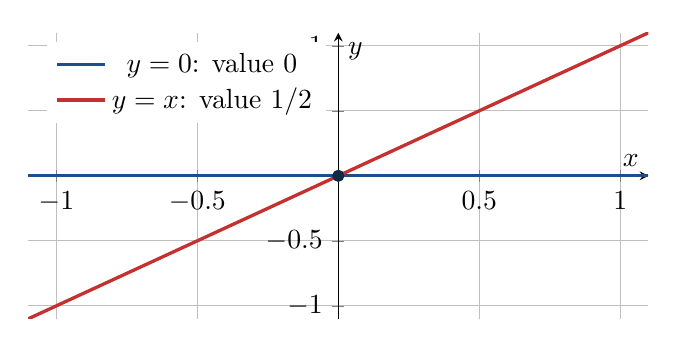
\begin{tikzpicture}[scale=1,>=Latex]
\begin{axis}[
  width=0.78\textwidth,height=0.43\textwidth,
  axis lines=middle,xmin=-1.1,xmax=1.1,ymin=-1.1,ymax=1.1,
  xlabel={$x$},ylabel={$y$},grid=both,
  legend style={draw=none,fill=white,at={(0.03,0.97)},anchor=north west}
]
\addplot[domain=-1.1:1.1,samples=2,ashblue,very thick] {0};
\addlegendentry{$y=0$: value $0$}
\addplot[domain=-1.1:1.1,samples=2,linered,very thick] {x};
\addlegendentry{$y=x$: value $1/2$}
\addplot[only marks,mark=*,mark size=2pt,navy] coordinates {(0,0)};
\end{axis}
\end{tikzpicture}
\end{center}

\begin{answerbox}
At the origin, \(f_x=f_y=0\). The directional derivative exists only in directions where \(ab=0\), and then it equals \(0\). The function is not continuous at the origin.
\end{answerbox}

\subsection{5(iv) \(\displaystyle f(x,y)=\frac{xy^2}{x^2+y^4}\), with \(f(0,0)=0\)}

\textbf{(a) Partial derivatives at the origin.} For the \(x\)-partial,
\[
f_x(0,0)=\lim_{h\to0}\frac{f(h,0)-f(0,0)}{h}=0.
\]
For the \(y\)-partial,
\[
f_y(0,0)=\lim_{h\to0}\frac{f(0,h)-f(0,0)}{h}=0.
\]
Thus both first-order partial derivatives exist at the origin and equal \(0\).

\textbf{(b) Directional derivative at the origin.} Let \(u=(a,b)\) be a unit vector. Then
\[
f(ha,hb)=\frac{(ha)(h^2b^2)}{h^2a^2+h^4b^4}
=\frac{h a b^2}{a^2+h^2b^4}.
\]
Therefore
\[
D_u f(0,0)=\lim_{h\to0}\frac{f(ha,hb)-0}{h}
=\lim_{h\to0}\frac{a b^2}{a^2+h^2b^4}.
\]
If \(a\neq0\), then
\[
D_u f(0,0)=\frac{b^2}{a}.
\]
If \(a=0\), then the path is the vertical axis and \(f(0,hb)=0\), so
\[
D_u f(0,0)=0.
\]
Thus all directional derivatives exist, but their values depend strongly on the direction.

\textbf{(c) Non-continuity at the origin.} Along the path \(x=y^2\),
\[
f(y^2,y)=\frac{y^2y^2}{y^4+y^4}=\frac12.
\]
Along the path \(y=0\),
\[
f(x,0)=0.
\]
The path-limits differ, so the full limit at the origin does not exist. Since \(f(0,0)=0\), the function is not continuous at the origin.

\begin{center}
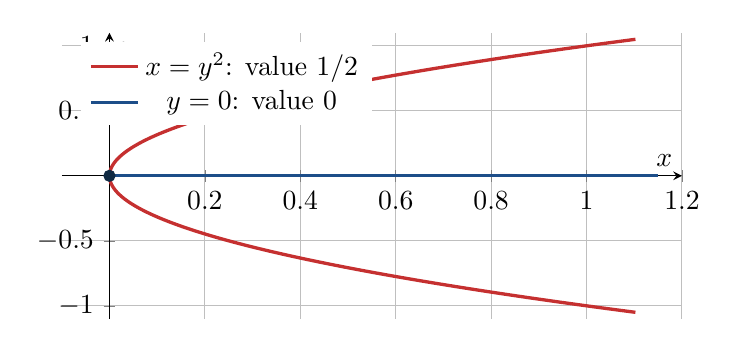
\begin{tikzpicture}[scale=1,>=Latex]
\begin{axis}[
  width=0.78\textwidth,height=0.43\textwidth,
  axis lines=middle,xmin=-0.1,xmax=1.2,ymin=-1.1,ymax=1.1,
  xlabel={$x$},ylabel={$y$},grid=both,
  legend style={draw=none,fill=white,at={(0.03,0.97)},anchor=north west}
]
\addplot[domain=-1.05:1.05,samples=160,linered,very thick] ({x^2},{x});
\addlegendentry{$x=y^2$: value $1/2$}
\addplot[domain=0:1.15,samples=2,ashblue,very thick] {0};
\addlegendentry{$y=0$: value $0$}
\addplot[only marks,mark=*,mark size=2pt,navy] coordinates {(0,0)};
\end{axis}
\end{tikzpicture}
\end{center}

\begin{answerbox}
\[
\boxed{f_x(0,0)=f_y(0,0)=0,\qquad
D_{(a,b)}f(0,0)=
\begin{cases}
\dfrac{b^2}{a},&a\neq0,\\[6pt]
0,&a=0,
\end{cases}}
\]
and \(f\) is not continuous at the origin.
\end{answerbox}

\section*{Summary table of main limit and derivative outcomes}
\addcontentsline{toc}{section}{Summary table of main outcomes}

\begin{center}
\renewcommand{\arraystretch}{1.25}
\begin{tabular}{@{}p{0.24\textwidth}p{0.48\textwidth}p{0.20\textwidth}@{}}
\toprule
Topic & Key computation & Outcome\\
\midrule
Line indicator at \((0,0)\) & line \(y=2x\) gives \(2\), other lines give \(0\) & full limit DNE\\
Line indicator at \((1,1)\) & positive distance from \((1,1)\) to \(y=2x\) & limit \(0\)\\
Parabola indicator on \(y=x^2\) & straight lines give \(0\), parabola gives \(2\) & full limit DNE on parabola\\
\(\frac{x^2-y^2}{x^2+y^2}\) & line \(y=mx\) gives \(\frac{1-m^2}{1+m^2}\) & no continuous extension\\
\(\frac{xy}{x^2+y^2}\) & coordinate partials exist, but diagonal path gives \(1/2\) & not continuous\\
\(\frac{xy^2}{x^2+y^4}\) & all directional derivatives exist, path \(x=y^2\) gives \(1/2\) & not continuous\\
\bottomrule
\end{tabular}
\end{center}

\end{document}
